\documentclass[dvips,xcolor=pst]{beamer}
%\documentclass[dvips,handout,xcolor=pst]{beamer}
%\documentclass[letterpaper]{article}
%\usepackage{beamerarticle}
\newcommand{\newblock}{}
\usepackage{pstricks}
%\usepackage{hyperref}
%\usepackage[authoryear]{natbib}
\usepackage{graphicx}
\usepackage{multimedia}
\usepackage{pgfpages}
\usepackage{arydshln}
\usepackage{commath}
\usepackage{vector}
%\usepackage{cancel}
\usepackage{ulem}
%\usepackage{times}

\graphicspath{{pysci_eps/}}

\newcommand{\defeq}{\ensuremath{\buildrel {\text{def}}\over{=}}} 

%\usetheme{Berlin}
%\usetheme{Boadilla}
%\usetheme{Luebeck}
%\usetheme{Pittsburgh}
\usetheme{CambridgeUS}
%\usecolortheme{seagull}
%\setbeameroption{show notes}
%\setbeameroption{show only notes}
%\pgfpagesuselayout{2 on 1}[letterpaper,border shrink=0.2in]

\title[Futuristic Computing with Python]{Futuristic Computing Platform for
Science and Engineering: Python + NumPy/SciPy/Matplotlib}
%
\author[\href{http://solvcon.net/yyc/}{Chen}]%
{\href{http://solvcon.net/yyc/}{Yung-Yu Chen} \\ {\scriptsize
\url{yyc@solvcon.net}}}
%
\institute[\href{http://solvcon.net/}{SOLVCON}]%
{\href{http://solvcon.net/}{SOLVCON Project}}
%
\date[2011/9/19]{September 19, 2011}

\begin{document}

\begin{frame}
\titlepage
\end{frame}

\section{Futuristic Scientific Computing}

\begin{frame}{
%
Python for Scientific and Engineering Computing
%
}
\begin{itemize}
  \item Productive.
  \item Robust.
  \item Maintainable.
  \item Reasonably fast.
\end{itemize}
\end{frame}

\section{High-Performance Computing}

\begin{frame}{
%
New Hardware Boosts Computing Power
%
}
\begin{center}
  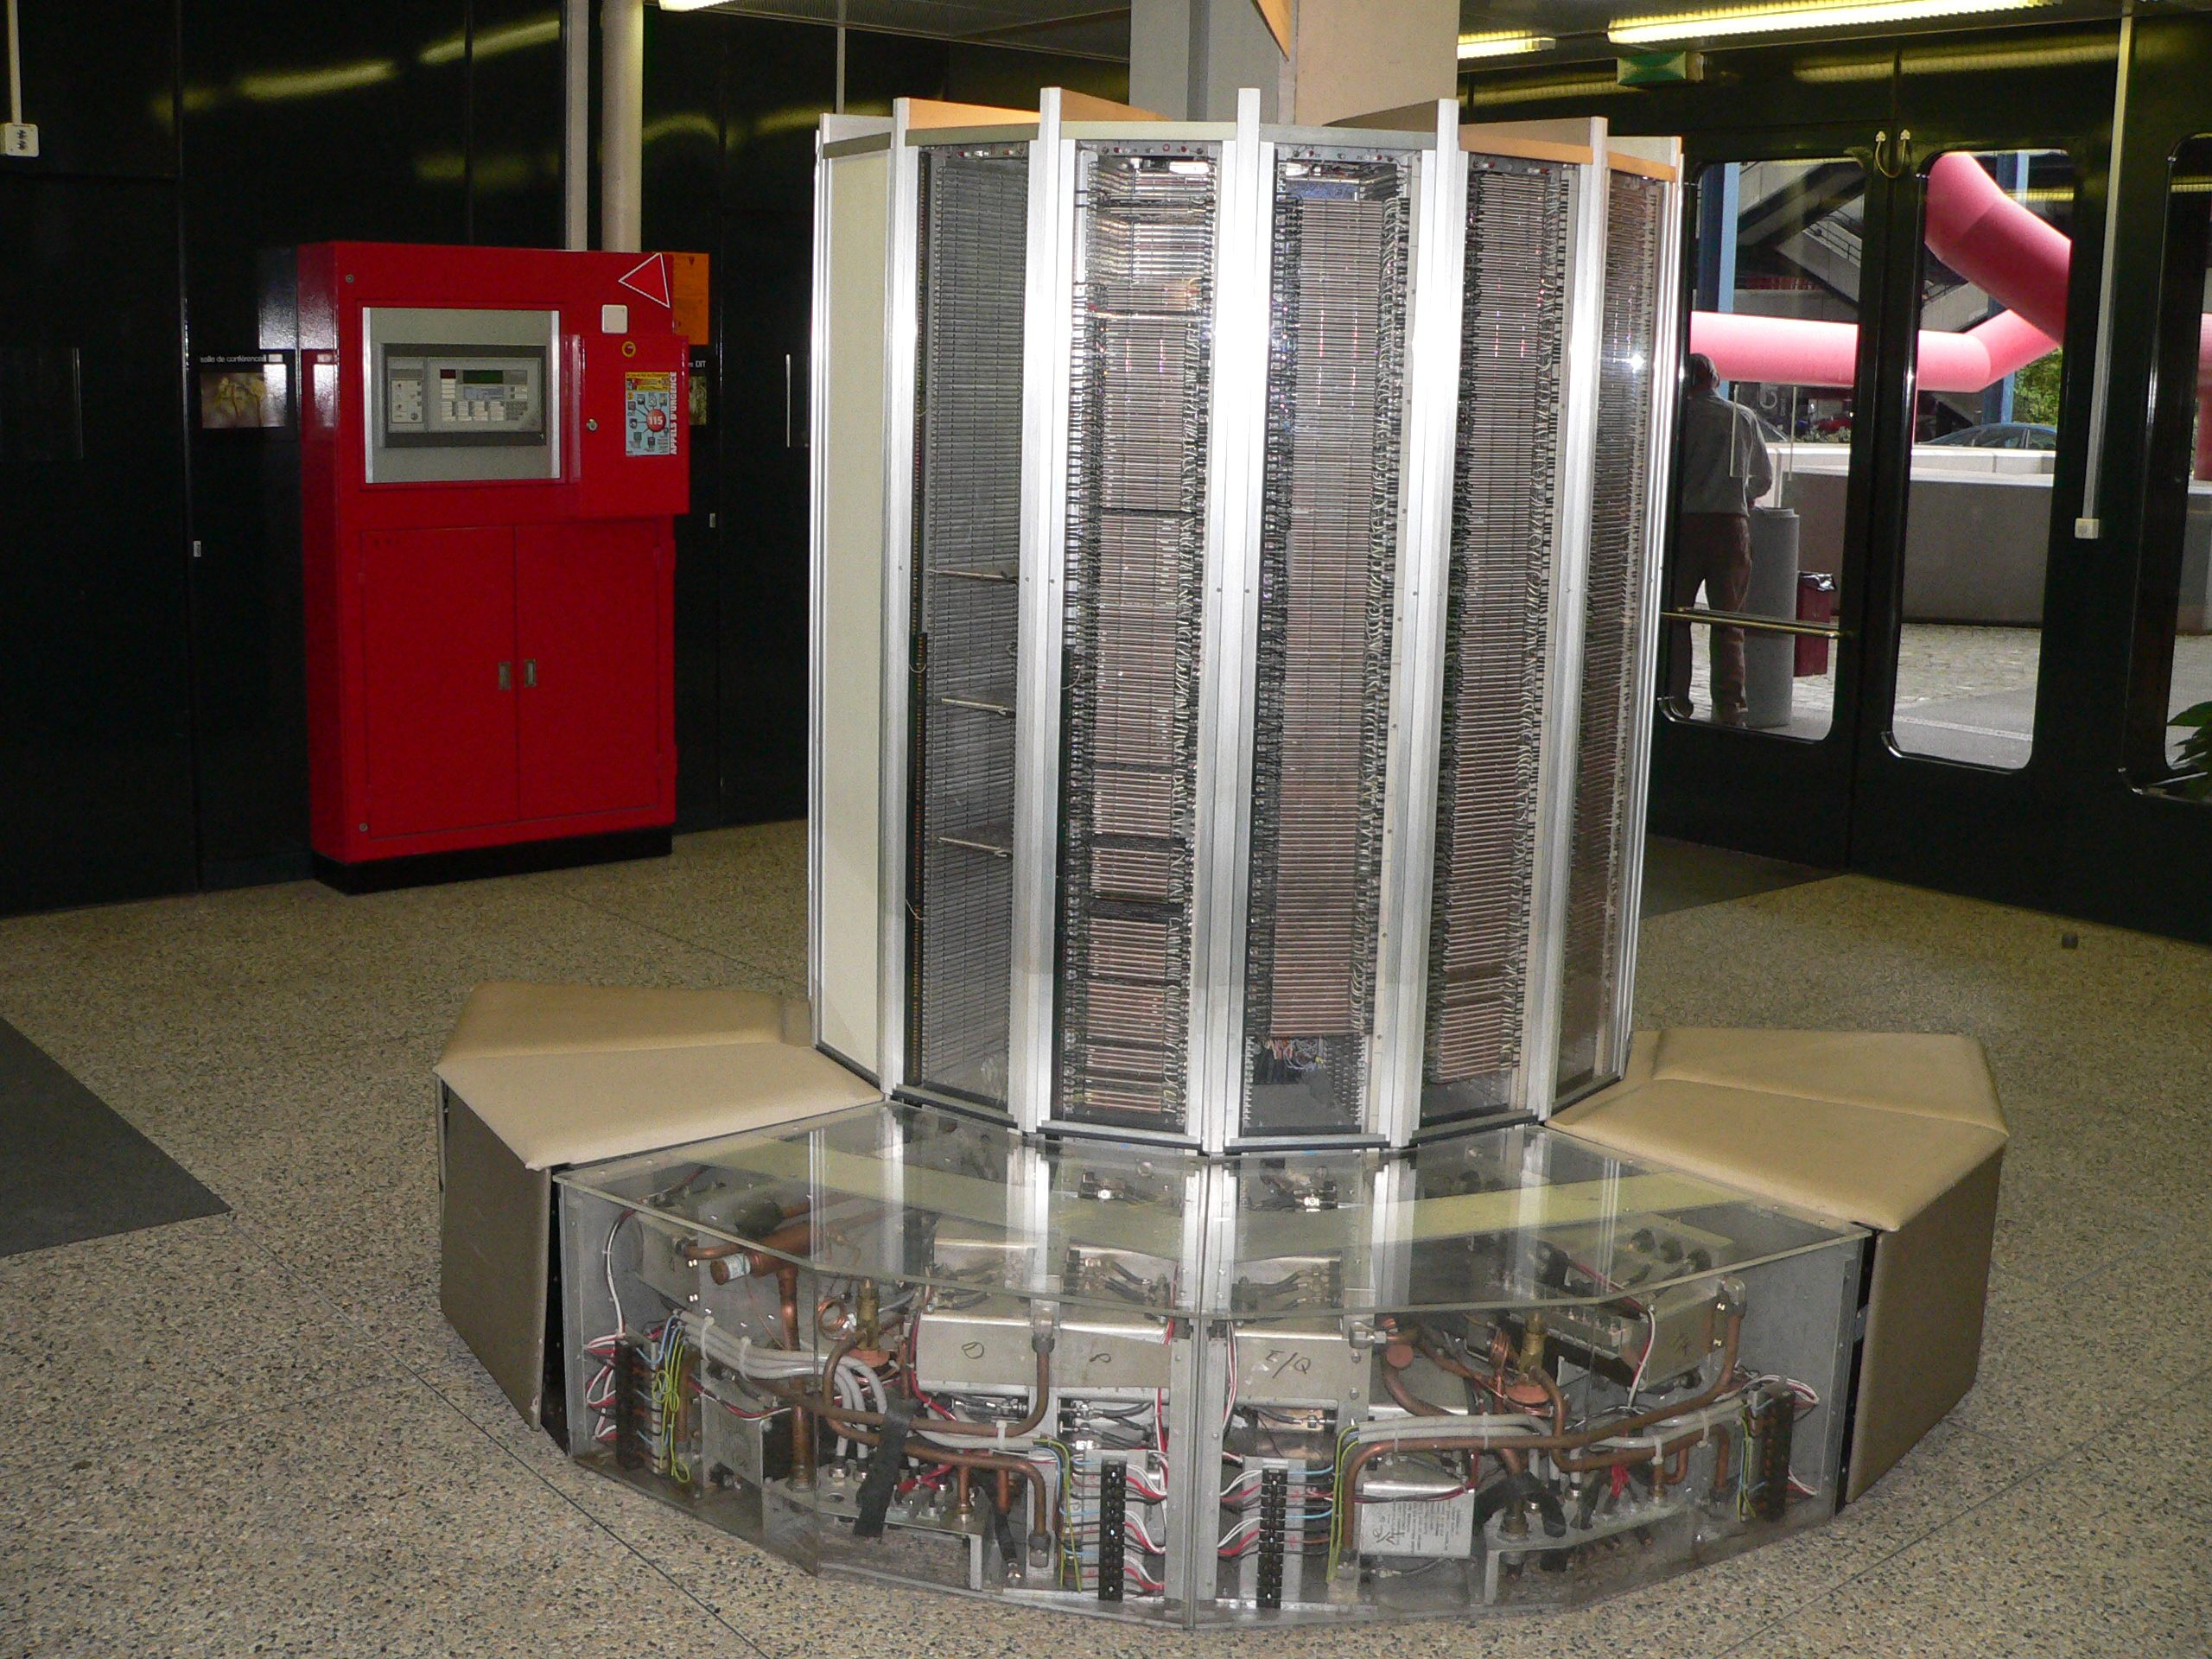
\includegraphics[height=0.3\textheight]{cray.eps}
  \hspace{0.01\textwidth}
  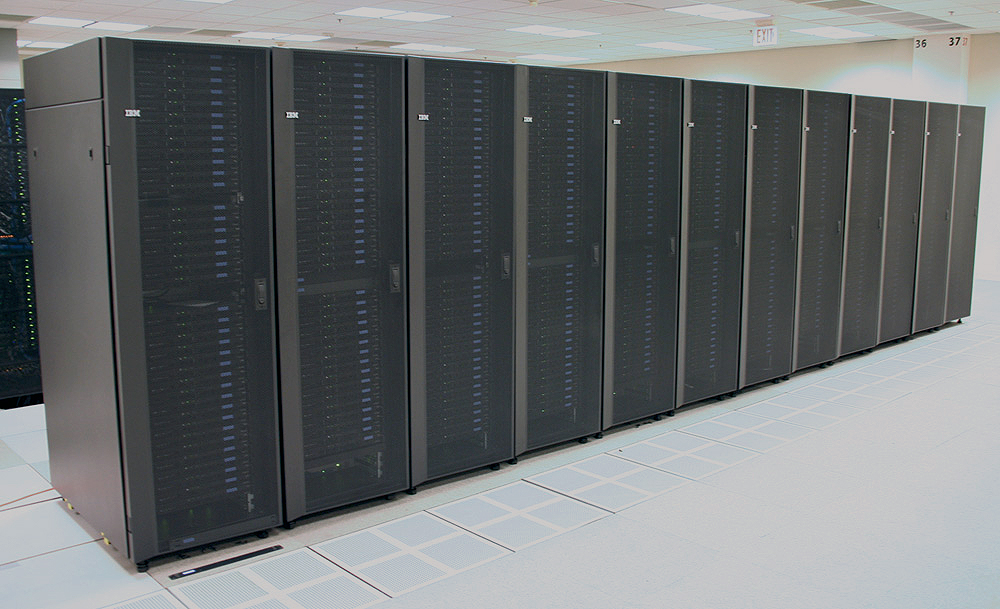
\includegraphics[height=0.3\textheight]{oscglenn.eps}
  \hspace{0.01\textwidth}
  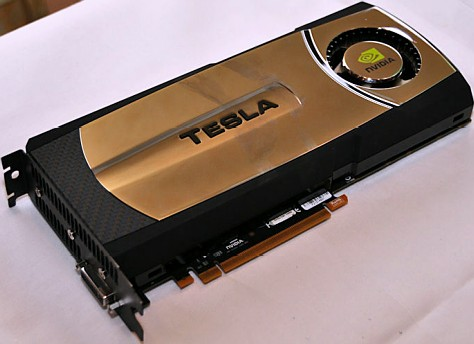
\includegraphics[height=0.3\textheight]{tesla_g300.eps}
\end{center}
\begin{itemize}
  \item 1970-1990: Vector machines (Cray computers).
  \item 1990-200x: Clusters with MPI.
  \item Now: Many-core technology, e.g., general-purpose GPU clusters.
\end{itemize}
\end{frame}

\begin{frame}{
%
Hybrid Parallel Computing
%
}
\begin{minipage}[c]{\textwidth}\centering
\parbox{0.3\textwidth}{\centering
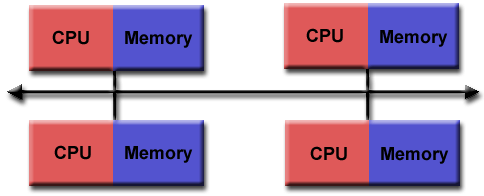
\includegraphics[width=0.3\textwidth]{mem_distributed.eps} \\ distributed
(cluster)}
+ 
\parbox{0.3\textwidth}{\centering 
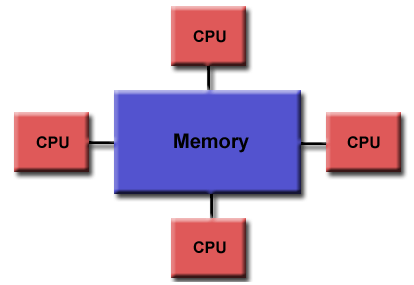
\includegraphics[width=0.3\textwidth]{mem_shared.eps} \\ shared (vector/GPU)}
= 
\parbox{0.3\textwidth}{\centering
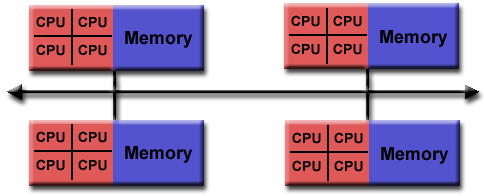
\includegraphics[width=0.3\textwidth]{mem_hybrid.eps} \\ hybrid (GPU cluster)}
\end{minipage}
\begin{itemize}
  \item Definition: Simultaneously use distributed-memory (e.g., MPI) and
  shared-memory (e.g., CUDA/OpenCL) parallel computing.
  \begin{itemize}
    \item The difference in parallel computing models requires using disparate
    programming tools.
  \end{itemize}
  \item Software structure needs to be organized to accommodate the different
  computing models.
\end{itemize}
\end{frame}

\begin{frame}{
%
Python Addresses the Challenges in HPC
%
} \large
\begin{itemize}
  \item Three challenges for the next-generation solvers of hyperbolic PDEs.
  \begin{itemize} \large
    \item \alert{Challenge 1}: HPC by using advanced hardware, e.g., GPGPU
    computing, CUDA/OpenCL, hybrid parallelism, etc.
    \item \alert{Challenge 2}: I/O and post-processing large data; the
    bottleneck is the laborious work flow for post-processing the results.
    \item \alert{Challenge 3}: Code reuse for long life cycle: Extend the
    technologies for various applications.
  \end{itemize}
  \item Python can address the challenges.
  \begin{itemize} \large
    \item SOLVCON is a successful prototype.
    \item NumPy is the foundation.
  \end{itemize}
\end{itemize}
\end{frame}

\section{Conclusions}

\begin{frame}{
%
Conclusions
%
}
\begin{itemize}
  \item De facto Python tool chain for scientific/engineering computing: NumPy
  + SciPy + Matplotlib.
\end{itemize}
\end{frame}

\end{document}

% vim: set spell:
